\documentclass[11pt]{article}
\usepackage{fancyhdr}\thispagestyle{empty}
\usepackage{amsmath}
\usepackage{tikz}
\usetikzlibrary{shapes.geometric, arrows.meta}

\topmargin      0.1in
\oddsidemargin  0in
\evensidemargin 0in
\textheight     8.80in
\textwidth      6.50in
\marginparsep   0.25cm
\headheight     0in
\headsep        0in

\tikzstyle{startstop} = [rectangle, rounded corners, minimum width=3cm,
  minimum height=1cm, text centered, draw=black, fill=red!30]
\tikzstyle{io} = [trapezium, trapezium stretches=true, trapezium left angle=70,
  trapezium right angle=110, minimum width=3cm, minimum height=1cm,
  text centered, draw=black, fill=blue!30]
\tikzstyle{process} = [rectangle, minimum width=3cm, minimum height=1cm,
  text centered, draw=black, fill=orange!30]
\tikzstyle{decision} = [diamond, minimum width=3cm, minimum height=1cm,
  text centered, draw=black, fill=green!30]
\tikzstyle{arrow} = [-{Latex[length=3mm]}]

\begin{document}
\begin{center}
{\Large {\tt namdcph} Execution Flow Chart}
\vspace{11pt}

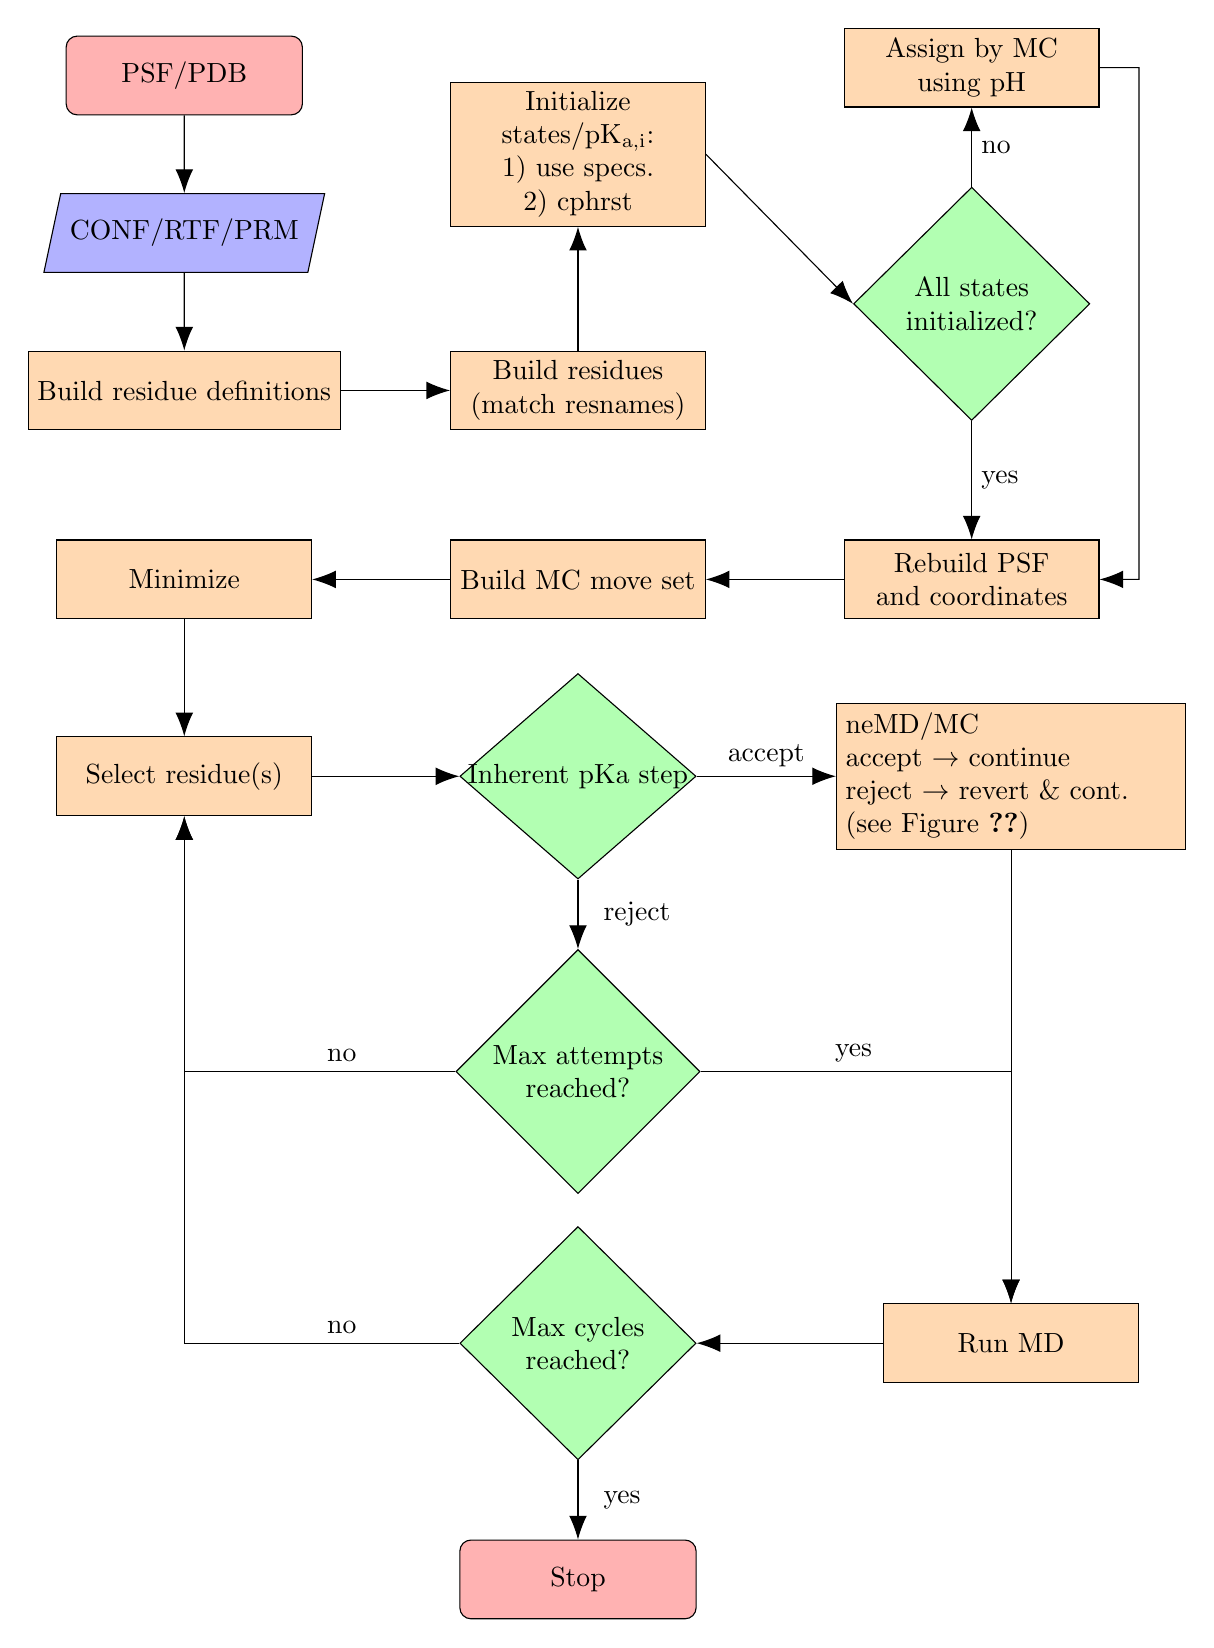
\begin{tikzpicture}[node distance=2cm]
  \node (start) [startstop] {PSF/PDB};
  \node (in1) [io, below of=start] {CONF/RTF/PRM};
  \node (pro1) [process, below of=in1] {Build residue definitions};
  \node (pro2) [process, right of=pro1, text width=3cm, xshift=3cm]
    {Build residues (match resnames)};
  \node (pro3) [process, right of=in1, text width=3cm,
    xshift=3cm, yshift=1cm] {Initialize states/pK$_{\text{a,i}}$:\\
    1) use specs.\\2) cphrst};
  \node (dec1) [decision, right of=pro2, text width=3cm, xshift=3cm,
    yshift=1.1cm, inner sep=-5pt] {All states initialized?};
  \node (pro4) [process, right of=pro3, xshift=3cm, text width=3cm,
    yshift=1.1cm] {Assign by MC using pH};
  \node (pro5) [process, below of=dec1, text width=3cm, yshift=-1.5cm]
    {Rebuild PSF and coordinates};
  \node (pro6) [process, left of=pro5, text width=3cm, xshift=-3cm]
    {Build MC move set};
  \node (pro7) [process, left of=pro6, text width=3cm, xshift=-3cm]
    {Minimize};
  \node (pro8) [process, below of=pro7, text width=3cm, yshift=-0.5cm]
    {Select residue(s)};
  \node (dec2) [decision, right of=pro8, text width=3cm, xshift=3cm,
    inner sep=-5pt] {Inherent pKa step};
  \node (dec3) [decision, below of=dec2, text width=3cm, yshift=-1.75cm,
    inner sep=-4pt] {Max attempts reached?};
  \node (pro9) [process, right of=dec2, text width=4.2cm, xshift=3.5cm,
    align=left]
    {neMD/MC\\
     accept $\rightarrow$ continue\\
     reject $\rightarrow$ revert \& cont.\\
     (see Figure~\ref{fig:namdcph_nemdmc})
    };
  \node (pro10) [process, below of=pro9, text width=3cm, yshift=-5.2cm]
    {Run MD};
  \node (dec4) [decision, left of=pro10, text width=3cm, xshift=-3.5cm,
    inner sep=-5pt] {Max cycles reached?};
  \node (stop) [startstop, below of=dec4, yshift=-1cm] {Stop};

  \draw [arrow] (start) -- (in1);
  \draw [arrow] (in1) -- (pro1);
  \draw [arrow] (pro1) -- (pro2);
  \draw [arrow] (pro2) -- (pro3);
  \draw [arrow] (pro3.east) -- (dec1.west);
  \draw [arrow] (dec1) -- node[anchor=west] {no} (pro4);
  \draw [arrow] (pro4.east) -- ++(0.5cm,0) -- ++(0,-6.5cm) -- (pro5.east);
  \draw [arrow] (dec1) -- node[anchor=west] {yes} (pro5);
  \draw [arrow] (pro5) -- (pro6);
  \draw [arrow] (pro6) -- (pro7);
  \draw [arrow] (pro7) -- (pro8);
  \draw [arrow] (pro8) -- (dec2);
  \draw [arrow] (dec2) -- node[anchor=west, xshift=0.2cm] {reject} (dec3);
  \draw [arrow] (dec2) -- node[anchor=south] {accept} (pro9);
  \draw [arrow] (dec3) -| node[anchor=south, xshift=2cm] {no} (pro8);
  \draw [arrow] (dec3) -| node[anchor=south, xshift=-2cm] {yes} (pro10);
  \draw [arrow] (pro9) -- (pro10);
  \draw [arrow] (pro10) -- (dec4);
  \draw [arrow] (dec4) -| node[anchor=south, xshift=2cm] {no} (pro8);
  \draw [arrow] (dec4) -- node[anchor=west, xshift=0.2cm] {yes} (stop);
\end{tikzpicture}
\end{center}

\end{document}
